% !Mode:: "TeX:UTF-8"
\documentclass[13pt]{ctexbeamer}


\usepackage{amsmath,amssymb,amsthm}             % AMS Math
\usepackage{graphicx}
\usepackage{epstopdf}
\usepackage{tikz}
\linespread{1.3}

\usepackage{mathrsfs}  %花写字母


%%%=== theme ===%%%
% \usetheme{Warsaw}
%\usetheme{Copenhagen}
%\usetheme{Singapore}
\usetheme{Madrid}
%\usefonttheme{professionalfonts}
%\usefonttheme{serif}
% \usefonttheme{structureitalicserif}
%%\useinnertheme{rounded}
%%\useinnertheme{inmargin}
\useinnertheme{circles}
%\useoutertheme{miniframes}
\setbeamertemplate{navigation symbols}{}
%\setbeamertemplate{footline}[page number]
\setbeamertemplate{footline}[frame number]


%\usepackage[fontset=mac]{ctex}
%\usepackage{ctex}


\usepackage{hyperref}
\usepackage{tipa}

\titlegraphic{
\includegraphics[width=2cm]{tjnu.jpg}}

\usepackage{color}
\definecolor{linkcol}{rgb}{0,0,0.4}
\definecolor{citecol}{rgb}{0.5,0,0}

\usepackage{xcolor}
\newcommand{\red}[1]{\textcolor{red}{#1}}
\newcommand{\blue}[1]{\textcolor{blue}{#1}}
\newcommand{\green}[1]{\textcolor{green}{#1}}


  \usepackage{graphicx}
  \DeclareGraphicsExtensions{.eps}
%   \usepackage[a4paper,pagebackref,hyperindex=true,pdfnewwindow=true]{hyperref}



\usepackage{tikz}
\usetikzlibrary{graphs, positioning, quotes, shapes.geometric}

\begin{document}



\title[让LaTeX跑起来]{论文写作指导  ---  让LaTeX跑起来}
\author[]{{\large 张彪} }
\institute[]{{\normalsize
		天津师范大学\\[6pt]
		zhang@tjnu.edu.cn}}

\date{}


%
%\AtBeginSection[]
%{
%\begin{frame}
%	\frametitle{Outline}
%	\tableofcontents[currentsection]
%\end{frame}
%\setcounter{exa}{0}
%\setcounter{equation}{0}
%}



\begin{frame}
\maketitle
\end{frame}


\begin{frame}
	\frametitle{\textcolor{orange}{Outline}}
	\tableofcontents
\end{frame}




\section{文献搜索}
\begin{frame}{文献搜索 -- 用好校园网络资源}
    \begin{itemize}
        \item VPN  -- 可以在校外使用校园网络

        \href{https://svpn.tjnu.edu.cn/}{https://svpn.tjnu.edu.cn/}

        \href{https://vpn.tjnu.edu.cn/}{https://vpn.tjnu.edu.cn/}




        \item 图书馆

        \href{https://tsg.tjnu.edu.cn/}{https://tsg.tjnu.edu.cn/}
    \end{itemize}
\end{frame}


\begin{frame}{文献搜索}
    \begin{itemize}

        \item 知网

        \href{https://www.cnki.net/}{https://www.cnki.net/}

        \item 万方数据

        \href{https://www.wanfangdata.com.cn/}{https://www.wanfangdata.com.cn/}


        \item 维普网

        \href{http://www.cqvip.com/}{http://www.cqvip.com/}

        \item Web of Science

        \href{https://www.webofknowledge.com/}{https://www.webofknowledge.com/}
    \end{itemize}

\end{frame}

\begin{frame}{文献搜索}
    \begin{itemize}
        \item
        百度学术

        \href{http://xueshu.baidu.com/}{http://xueshu.baidu.com/}




        \item
        谷歌学术镜像

        \href{http://scholar.hedasudi.com/}{http://scholar.hedasudi.com/}

        \href{http://scholar.scqylaw.com/}{http://scholar.scqylaw.com/}

        \item
        Bing

        \item 俄罗斯搜索
    \end{itemize}

\end{frame}


\section{LaTeX}

\subsection{LaTex 简介}
\begin{frame}
	\begin{itemize}
	\item 	TeX
($\backslash$t\textepsilon x$\backslash$,常被读作$\backslash$t\textepsilon k$\backslash$,音译“泰赫”,“泰克”,写作“TEX”)

\item 它在学术界特别是数学、物理学和计算机科学界十分流行。
	\item
TeX被普遍认为是一个优秀的排版工具,尤其是对于复杂数学公式的处理。
	\item
科研工作者使用文本编辑器(WinEdt, TexStudio等)编写tex源文件(.tex),  经过LaTeX进行编译,能够排版出精美的pdf文件。
\end{itemize}

\begin{figure}

	\begin{tikzpicture}

	\tikzstyle{arrow} = [thick,->,>=stealth]
	\node[diamond, minimum width=3cm,
	minimum height=1cm, text width=2cm, rounded corners, text centered, fill=blue!30]     (tex)  {.tex文件};
	\node[diamond, rounded corners, minimum width=3cm,
	minimum height=1cm, text width=2cm, fill=blue!30, text centered,  right=100pt of tex]     (pdf)  {.pdf文档};
\draw [arrow] (tex) -- node[anchor=south] {LaTeX编译} (pdf);

\end{tikzpicture}
\end{figure}

\end{frame}


\begin{frame}{TeX}


	\begin{columns}[c]  %开始进入分栏环境,居中设置

		\column{6cm}

		\begin{itemize}
			\item
			TeX
			是一个由美国计算机教授高德纳(Donald Ervin Knuth)编写的排版软件。

			\item 高德纳最早开始自行编写TeX的原因,是因为当时的电脑排版技术十分粗糙,已经影响到他的巨著《计算机程序设计艺术》的印刷质量。作为一名计算机学家,他决定自行编写一个排版软件:TeX。
		\end{itemize}


		%\rightline{ {\Large 一华罗庚 \qquad \qquad\qquad}}
		\column{5cm}
		\begin{figure}[p]
			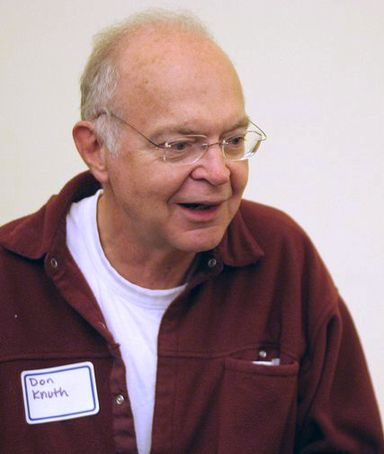
\includegraphics[scale=0.5]{Knuth.jpg}
			\caption{Donald Knuth(1938-~~)}
		\end{figure}

	\end{columns}


\end{frame}


\begin{frame}{LaTeX}
	\begin{columns}[c]  %开始进入分栏环境,居中设置

		\column{6cm}

\begin{itemize}
		\item LaTeX使用TeX作为它的格式化引擎,当前的版本是LaTeX2e(写作“LATEX2ε”)。

	\item LaTeX 由美国计算机科学家Leslie~ Lamport~(2013年获图灵奖)在20世纪80年代初期开发。
	\item 利用这种格式系统的处理,即使用户没有排版和程序设计的知识也可以充分发挥由TEX所提供的强大功能。
\end{itemize}


		\column{5cm}
		\begin{figure}[p]
			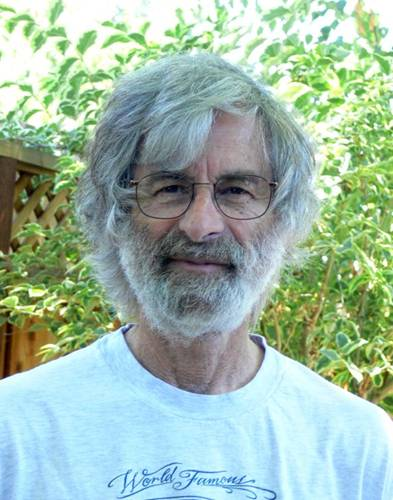
\includegraphics[scale=0.4]{Lamport.jpg}
			\caption{Lamport(1941-~~)}
		\end{figure}

	\end{columns}


\end{frame}


%\begin{frame}{LaTeX}
%
%\begin{itemize}
%\item     LaTeX 是 基于 TeX 的排版系统。
%
%\item 实际上 LaTeX 利用 TeX 的控制命令,定义了许多新的控制命令并封装成一个可执行文件。
%
%\item这个可执行文件会去解释 LaTeX 新定义的命令成为 TeX 的控制命令,并最终交由 TeX 引擎进行排版。
%
%\item LaTeX 实际上是一个工具,它将用户按照它的格式编写的文档解释成 TeX 引擎能理解的形式并交付给 TeX 引擎处理,再将最终结果返回给用户。
%\end{itemize}
%
%
%
%
%\end{frame}



\begin{frame}{LaTeX 发音和书写}
	\begin{itemize}
\item 	由于TEX一词应该读作“泰赫”($\backslash$t\textepsilon x$\backslash$),所以LATEX一词可以音译为“拉泰赫”。
\item
	在英语中,IATEX实际通常读作
$\backslash$le\i t\textepsilon k$\backslash$
(音译“莱泰克”)或者(音译“拉泰克”)
$\backslash$l\textscripta\textlengthmark t\textepsilon k$\backslash$
\item
	LATEX的开发者Lamport表示对LATEX的读音没有偏好。
		\end{itemize}
	\vspace{15pt}
		\begin{itemize}
\item
LaTeX的正确的写法是
\begin{center}

\includegraphics[scale=0.08]{LATEX.jpg}
\end{center}
如果因技术限制而无法做到,则应该写成“LaTeX”。
\item
不得改变任何一个字母的大小写,以免和“latex” (乳胶) 混淆。
	\end{itemize}
\end{frame}






\begin{frame}{线上Latex:  Overleaf}
    网站
    \href{https://www.overleaf.com?r=4c8832b9&rm=d&rs=b
    }{https://www.overleaf.com/
    }


    \begin{itemize}
        \item 在线编辑

        \item 免安装,免配置

        \item 多人协作

        \item 版本管理
    \end{itemize}
\end{frame}



\begin{frame}{换行和新的段落}
    \begin{itemize}
        \item 一个空行或者多个连续空行代表着前后内容是两段,会产生缩进。


        \item  $\backslash\backslash$ 也可以表示换行,但只是换行,不会产生缩进。


        \item 一般是用插入空行来实现分段,为保证源文件的清晰

    \end{itemize}
\end{frame}

\begin{frame}{输入数学公式}

    欧拉函数常用于数论中.
    \begin{align}\label{eq1}
        \varphi(n)=n\left(1-\frac{1}{p_{1}}\right)\left(1-\frac{1}{p_{2}}\right) \cdots\left(1-\frac{1}{p_{q}}\right)
    \end{align}

    例如,若 $n=12=2^{2} \cdot 3$,则由\eqref{eq1}可得
    $$
    \varphi(12)=12\left(1-\frac{1}{2}\right)\left(1-\frac{1}{3}\right)=4
    $$


\end{frame}

\begin{frame}
    \begin{itemize}
        \item 插入图片
        \begin{center}
            
\includegraphics[width=2cm]{tjnu.jpg}
        \end{center}

        \item 插入表格
        \begin{table}
            \centering
            \caption{顾客损失率计算参数值}
            \begin{tabular}{|l||c|c|c|}
                \hline
                姓名 & 语文 & 数学 & 外语  \\
                \hline  \hline
                张三 & 87 & 100 & 93 \\
                \hline
                李四 & 75 & 64 & 52  \\
                \hline
                王二 & 80 & 82 & 78  \\
                \hline
            \end{tabular}
        \end{table}
    \end{itemize}



\end{frame}




    \begin{frame}{推荐使用TeXLive + TeXStudio }
    	推荐安装\green{最新版本}的

    	\begin{itemize}
    		\item \blue{TeXLive}  ---\red{发行版}

    		\href{https://www.tug.org/texlive/}{https://www.tug.org/texlive/}



    		\item \blue{TeXStudio}    ---\red{编辑器}

    		http://www.texstudio.org/
    	\end{itemize}

    	{TeXLive} + {TeXStudio}   ~安装指南,可以参考
    	\begin{itemize}
    		\item 	\href{https://zhuanlan.zhihu.com/p/80603542}{https://zhuanlan.zhihu.com/p/80603542}
    		\item \href{https://blog.csdn.net/yeler082/article/details/80665186}{https://blog.csdn.net/yeler082/article/details/80665186}
    	\end{itemize}
    \end{frame}

\subsection{LaTeX发行版与编辑器}
\begin{frame}{LaTeX发行版}
\begin{itemize}
	\item MiKTex
		\begin{itemize}
	\item
	MiKTeX 是 mick-tech 公司 TEX/LATEX 最新的
实施方案及相关程序 MiKTEX 集成软件包
管理器可以从互联网中安装缺失的部分宏
包。
\end{itemize}
	\item CTeX中文套装 (基于MiKTeX,支持中文,\green{已停更})

	\item \blue{TeX Live}   多数国外期刊采用的编译套装, \red{推荐安装}


	\item MacTeX -- macOS(OS X)系统下的一个定
制化的 TeXLive 版本。

\item proTeXt -- 基于 MikTeX 并把 TeXStudio 作为前端编辑器
\end{itemize}
\end{frame}


\begin{frame}{TeX Live}
	\begin{itemize}
		\item TeX Live 是 TUG (TeX User Group) 维护和发布的 TeX 系统,可说是「官方」的 TeX 系统。

	TeX Live包含与TeX系统相关的各种程序、编辑与查看工具、常用宏包及文档、常用字体及多国语言支持。
	\item
	TeX Live是许多Linux/Unix系统默认或推荐的TeX套装,同时也支持包括Windows和Mac OS X等在内的其它操作系统。
\end{itemize}
\begin{itemize}

%	\item 我们推荐任何阶段的 TeX 用户,都尽可能使用 TeX Live,以保持在跨操作系统平台、跨用户的一致性。
	\item TeX Live 的官方站点是 \href{https://tug.org/texlive/}{https://tug.org/texlive/}
	\item 建议尝试使用国内大学的镜像站下载。

	\href{https://mirrors.ustc.edu.cn/CTAN/systems/texlive/Images/} {https://mirrors.ustc.edu.cn/CTAN/systems/texlive/Images/}


	\href{https://mirrors.tuna.tsinghua.edu.cn/CTAN/systems/texlive/Images/}{https://mirrors.tuna.tsinghua.edu.cn/CTAN/systems/texlive/Images/}

\end{itemize}
\end{frame}


\begin{frame}{编辑器}
\begin{itemize}
\item  \blue{TeXStudio} (\red{推荐使用},开源)
\item TeXmaker
\item TeXworks (TexLive自带)
\item TexPad (for Mac users)
\item WinEdt (建议使用最新版,需要\green{破解})
\end{itemize}
\end{frame}






\subsection{中文排版}

%
%\begin{frame}{中文排版}
%\begin{itemize}
%    \item 最初,TeX 最初的开发者并没有考虑到中日韩等字符的处理,而只支持 ASCII 字符。
%    \item 在 XeTeX 出现之前,为了能让 TeX 系统排版中文,国人曾使用了 天元、CCT、CJK 等手段处理中文。其中 天元和 CCT 现在已经基本不用,CJK 因为使用时间长且效果相对较好,现在还有少数人使用。
%
%    \end{itemize}
%\end{frame}
%



\begin{frame}{CTeX 中文套装}


	\begin{itemize}
		\item
		CTeX 中文套装是中科院吴凌云研究员开发的一种LaTeX发行版。

		\item
		CTeX 中文套装 在MiKTeX的基础上增加了对中文的完整支持。

		\item CTeX 中文套装集成了WinEdt, SumatraPDF等工具软件。
		\item
		网站  http://www.ctex.org/
		%	\item CTeX 套装是科学院吴凌云研究员的个人作品。


	\end{itemize}
	在 CTeX 套装刚刚问世之时,因其解决了中文的排版问题,所以广受欢迎。 但是,
	\begin{itemize}
		\item  一方面 CTeX 套装已经很久不更新(最新的稳定版本	v2.9.2.164 -- 2012.03.22),内里的宏包、工具陈旧;
		\item 另一方面,XeLaTeX等技术逐渐成熟,可以更简便地完成中文排版;
	\end{itemize}

	因此,\red{不推荐使用 CTeX 中文套装},除非作为\blue{老中文期刊的备选版本}。

	%不要安装和使用 CTeX 套装!
	%如\documentclass{ctexart}
\end{frame}


\begin{frame}{XeTeX}

	\begin{itemize}
		\item 不同于 CJK 等方式使用 TeX 和 pdfTeX 这两个不直接支持 Unicode 字符的引擎,\blue{XeTeX 引擎}直接支持 Unicode 字符。也就是说现在不使用 CJK 也能排版中日韩文的文档了,并且这种方式要比之前的方式更加优秀。

		\item XeLaTeX 和 XeTeX 的关系与 pdfLaTeX 和 pdfTeX 的关系类似,这里不再赘述。

		\item  使用 XeTeX 引擎需要使用 \red{UTF-8 编码}。{UTF-8 编码}是 Unicode 编码的一种。
	\end{itemize}
\end{frame}




\begin{frame}{CTeX 宏集}
	\begin{itemize}
		\item
		虽然它的名字也是「CTeX」,但是 CTeX 宏集和 CTeX 套装是两个不同的东西。
		\item  CTEX 宏集支持LATEX、pdfLATEX、XƎLATEX、LuaLATEX、upLATEX 等多种不同的编译方式,并为它们提供了统一的界面。主要功能由宏包  \blue{ctex} 以及中文文档类  \blue{ctexart}、\blue{ctexbook} 和  \blue{ctexbeamer}  等 实现。
		%{ctexrep}
		\item 我们推荐\red{使用 CTeX 宏集处理中文}。
		\item 中文的文档可以直接\red{使用ctex 文档类}。
		%也就是ctexart、ctexrep、ctexbook、ctexbeamer 这些。
	\end{itemize}


	%请在任何情况下优先使用 CTeX 宏集在 LaTeX 中处理中文!
\end{frame}



\subsection{网络资源}




\begin{frame}{如何克服LaTex使用中的困难}
	\begin{itemize}
\item 	  在使用中学习, 通过网络寻求帮助

\item 	  错误难找: 慢慢积累经验

\item 	  遇到问题怎么办?---  丰富的网络资源

	\end{itemize}


\begin{itemize}
    \item
   \blue{ \href{https://www.latexstudio.net/}{https://www.latexstudio.net/} }   ---     \red{Latex工作室}
    \item
    \href{https://www.overleaf.com?r=4c8832b9&rm=d&rs=b
}{https://www.overleaf.com/
}   ---  Overleaf
\item
http://www.latextemplates.com --- 各种模板

\end{itemize}
\end{frame}


\section{Mathpix Snip --- 数学公式识别神器}
\begin{frame}{Mathpix Snip --- 数学公式识别神器}
\begin{itemize}
	\item 截图识别公式,一键转换成 LaTeX 代码。

\href{https://mathpix.com/}{https://mathpix.com/}



$$
\varphi(n)=n\left(1-\frac{1}{p_{1}}\right)\left(1-\frac{1}{p_{2}}\right) \cdots\left(1-\frac{1}{p_{q}}\right)
$$

$$
\left\{\begin{array}{l}
    t_{\mathrm{a}}(t)=\frac{t_{\mathrm{amax}}+t_{\mathrm{amin}}}{2}+\frac{t_{\mathrm{amax}}-t_{\mathrm{amin}}}{2} \sin \frac{(h+18) \pi}{16} \quad(0 \leqslant h<6) \\
    t_{\mathrm{a}}(t)=\frac{t_{\mathrm{amax}}+t_{\mathrm{amin}}}{2}+\frac{t_{\mathrm{amax}}-t_{\mathrm{amin}}}{2} \sin \frac{(h-10) \pi}{8} \quad(6 \leqslant h<14) \\
    t_{\mathrm{a}}(t)=\frac{t_{\mathrm{amax}}+t_{\mathrm{amin}}}{2}+\frac{t_{\mathrm{amax}}-t_{\mathrm{amin}}}{2} \sin \frac{(h-6) \pi}{16} \quad(14 \leqslant h<24)
\end{array}\right.
$$

\end{itemize}
\end{frame}


\section{Tables Generator --- 表格识别神器 }
\begin{frame}{Tables Generator  --- 表格识别神器 }
\begin{itemize}
	\item 	 像在 Excel 里一样使用表格,一键转换成 LaTeX 代码。
	\href{ http://www.tablesgenerator.com/}{ http://www.tablesgenerator.com/}

\end{itemize}
\begin{table}[]
    \caption{题目}
    \centering
    \begin{tabular}{|c|c|c|c|c|c|c|}
        \hline
        & 0 & 1    & 2  & 3  & 4   & 5 \\ \hline
        0 & 1 & 33   &    &    &     &   \\ \hline
        0 & 1 & 113  &    & 34 &     &   \\ \hline
        2 & 1 & 2343 & 1  &    & 34  &   \\ \hline
        3 & 1 & 3    & 3  & 1  & 343 &   \\ \hline
        4 & 1 & 4    & 6  & 4  & 1   &   \\ \hline
        5 & 1 & 5    & 10 & 10 & 5   & 1 \\ \hline
    \end{tabular}
\end{table}


\end{frame}


\section{JabRef --- 文献管理软件}
\begin{frame}{JabRef  --- 文献管理软件}
\begin{itemize}
\item  JabRef

\href{https://www.jabref.org/}{https://www.jabref.org/}
\end{itemize}
\end{frame}
\end{document}